\tikzset{every picture/.style={line width=0.75pt}} %set default line width to 0.75pt        

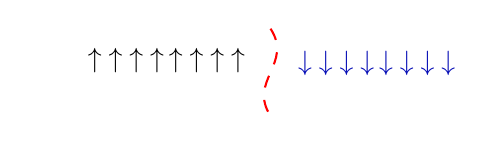
\begin{tikzpicture}[x=0.75pt,y=0.75pt,yscale=-1,xscale=1]
%uncomment if require: \path (0,241); %set diagram left start at 0, and has height of 241

%Shape: Boxed Bezier Curve [id:dp7848819814242627] 
\draw [color={rgb, 255:red, 255; green, 0; blue, 0 }  ,draw opacity=1 ] [dash pattern={on 4.5pt off 4.5pt}]  (197.51,67.6) .. controls (208.5,84.4) and (186.52,92.8) .. (197.51,109.6) ;

% Text Node
\draw (108,75.57) node [anchor=north west][inner sep=0.75pt]    {$\uparrow $};
% Text Node
\draw (128,75.57) node [anchor=north west][inner sep=0.75pt]    {$\uparrow $};
% Text Node
\draw (118,75.57) node [anchor=north west][inner sep=0.75pt]    {$\uparrow $};
% Text Node
\draw (138,75.57) node [anchor=north west][inner sep=0.75pt]    {$\uparrow $};
% Text Node
\draw (147,75.57) node [anchor=north west][inner sep=0.75pt]    {$\uparrow $};
% Text Node
\draw (167,75.57) node [anchor=north west][inner sep=0.75pt]    {$\uparrow $};
% Text Node
\draw (157,75.57) node [anchor=north west][inner sep=0.75pt]    {$\uparrow $};
% Text Node
\draw (177,75.57) node [anchor=north west][inner sep=0.75pt]    {$\uparrow $};
% Text Node
\draw (219,91.77) node [anchor=north east][inner sep=0.75pt]  [color={rgb, 255:red, 7; green, 14; blue, 182 }  ,opacity=1 ,rotate=-180,xscale=-1]  {$\uparrow $};
% Text Node
\draw (239,91.77) node [anchor=north east][inner sep=0.75pt]  [color={rgb, 255:red, 7; green, 14; blue, 182 }  ,opacity=1 ,rotate=-180,xscale=-1]  {$\uparrow $};
% Text Node
\draw (229,91.77) node [anchor=north east][inner sep=0.75pt]  [color={rgb, 255:red, 7; green, 14; blue, 182 }  ,opacity=1 ,rotate=-180,xscale=-1]  {$\uparrow $};
% Text Node
\draw (249,91.77) node [anchor=north east][inner sep=0.75pt]  [color={rgb, 255:red, 7; green, 14; blue, 182 }  ,opacity=1 ,rotate=-180,xscale=-1]  {$\uparrow $};
% Text Node
\draw (258,91.77) node [anchor=north east][inner sep=0.75pt]  [color={rgb, 255:red, 7; green, 14; blue, 182 }  ,opacity=1 ,rotate=-180,xscale=-1]  {$\uparrow $};
% Text Node
\draw (278,91.77) node [anchor=north east][inner sep=0.75pt]  [color={rgb, 255:red, 7; green, 14; blue, 182 }  ,opacity=1 ,rotate=-180,xscale=-1]  {$\uparrow $};
% Text Node
\draw (268,91.77) node [anchor=north east][inner sep=0.75pt]  [color={rgb, 255:red, 7; green, 14; blue, 182 }  ,opacity=1 ,rotate=-180,xscale=-1]  {$\uparrow $};
% Text Node
\draw (288,91.77) node [anchor=north east][inner sep=0.75pt]  [color={rgb, 255:red, 7; green, 14; blue, 182 }  ,opacity=1 ,rotate=-180,xscale=-1]  {$\uparrow $};
% Text Node
\draw (81,87.4) node [anchor=north west][inner sep=0.75pt]    {$\dotsc $};
% Text Node
\draw (288,84.4) node [anchor=north west][inner sep=0.75pt]  [color={rgb, 255:red, 19; green, 101; blue, 198 }  ,opacity=1 ]  {$\dotsc $};


\end{tikzpicture}